\documentclass[12pt]{article}
\usepackage{../preamble3}
%\pagenumbering{gobble}
\title{Math Miscellani}
\author{James \& Patrick}
\date{Revised:~\today}


\begin{document}
\maketitle
\begin{minipage}{\textwidth}
\begin{abstract}\setlength{\parindent}{0pt}%
This note reviews tips and tricks and selected problems to prepare for middle school math competitions. Written for personal use. Please report typos and errors over at \url{https://github.com/ptoche/Math/tree/master/mathcounts}. 
\end{abstract}
\end{minipage}

\thispagestyle{empty}
\clearpage

%%%%%%%%%%%%%%%%%%%%%%%%%%%%%%%%%%%%%%%%%%%%%%%%%%%%%%%%%%%%%%%%%%%%%%%%
\subsection*{Triangle}
Height and Area of an equilateral triangle with side $a$.

\begin{answer}
Let $A$ denote the area, and $h$ the height of the triangle. 
\begin{center}
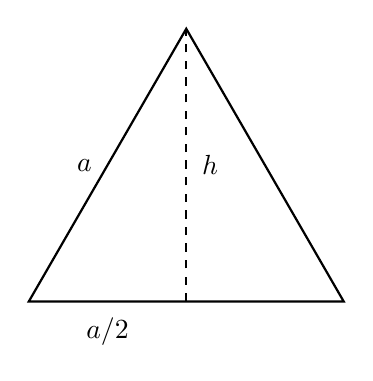
\begin{tikzpicture}[thick, sharp corners, inner sep=1mm, outer sep =1mm, scale=4]
\draw (0,0) -- (0.5,0) node[midway,below]{$a/2$} -- (1,0) -- (0.5, 0.866) -- cycle node[midway,left]{$a$}; 
\draw[dashed] (0.5,0) -- (0.5,0.866) node[midway,right]{$h$};
\end{tikzpicture}
\end{center}
The area of the triangle is given by one-half the product of the base and height:
\begin{align*}
A = \frac{1}{2} ah
\end{align*}
The height $h$ is unknown, but can be found by an application of the Pythagoras theorem.
\begin{align*}
& h^2 + \left(\frac{a}{2}\right)^2 = a^2 \\
\Rightarrow
h^2 & = a^2 - \frac{a^2}{4} 
      = \frac{3a^2}{4}
\end{align*}
And thus,
\begin{empheq}[box={\mathbox[colback=white]}]{equation*}
    h = \frac{a}{2} \sqrt{3}
\end{empheq}
\begin{empheq}[box={\mathbox[colback=white]}]{equation*}
    A = \left(\frac{a}{2}\right)^2 \sqrt{3}
\end{empheq}
\end{answer}
%%%%%%%%%%%%%%%%%%%%%%%%%%%%%%%%%%%%%%%%%%%%%%%%%%%%%%%%%%%%%%%%%%%%%%%%

\iftoggle{showAnswers}{\newpage}

%%%%%%%%%%%%%%%%%%%%%%%%%%%%%%%%%%%%%%%%%%%%%%%%%%%%%%%%%%%%%%%%%%%%%%%%
\subsection*{From Words to Equations}
There were $9$ adults and $11$ children at the movie at $11{:}45$a.m. By $11{:}50$a.m., $7$ more adults and $8$ more children were at the movie. At $12{:}00$p.m., there were $60$ adults and children, and the ratio of adults to children was the same as at $11{:}45$a.m. How many more children came to the movie between $11{:}50$a.m. and $12{:}00$p.m.?

\begin{answer}
Let $a$ denote the number of adults and $c$ denote the number of children, who came to the movie between $11{:}50$a.m. and $12{:}00$p.m.
\begin{align*}
a + c & = 25 \\
\frac{a + 16}{c + 19} & = \frac{9}{11}
\end{align*}
This is a system of two equations in two unknowns, $a$ and $c$. After a simple transformation, the second equation becomes linear in $a$ and $c$.
\begin{align*}
a + c & = 25 \\
11 (a + 16) & = 9 (c + 19) \Rightarrow 11a - 9c = 9 \cdot 19 - 11 \cdot 16
\end{align*}
Since we are interested in solving for $c$, let's substitute $a$ out:
\begin{align*}
11 (25-c) - 9c & = 9 \cdot 19 - 11 \cdot 16 \\
\Rightarrow 
c & = \frac{11 \cdot 25 + 11 \cdot 16 - 9 \cdot 19}{20} 
    = \frac{11 \cdot 41 - 9 \cdot 19}{20} 
    = \frac{410 + 41 - 190 + 19}{20} \\
  & = \frac{280}{20} = 14 \\
\Rightarrow 
a & = 25 - 14 = 11
\end{align*}        
\begin{empheq}[box={\mathbox[colback=white]}]{equation*}
    11 ~\text{children}
\end{empheq}
\end{answer}
%%%%%%%%%%%%%%%%%%%%%%%%%%%%%%%%%%%%%%%%%%%%%%%%%%%%%%%%%%%%%%%%%%%%%%%%

\iftoggle{showAnswers}{\newpage}

%%%%%%%%%%%%%%%%%%%%%%%%%%%%%%%%%%%%%%%%%%%%%%%%%%%%%%%%%%%%%%%%%%%%%%%%
\subsection*{Quadratic Equations}
The sum of a number $x$ and its reciprocal equals $-\dfrac{17}{4}$. What is the sum of all possible values of $x$? Express your answer as a common fraction. 

\begin{answer}
The possible values of $x$ satisfy:
\begin{align*}
x + \frac{1}{x} = -\frac{17}{4}
\end{align*}
This is a quadratic equation in disguise. Multiply through by $x$:
\begin{align*}
x^2 + 1 = -\frac{17}{4} x
\end{align*}
Rearrange to obtain the standard display format:
\begin{align*}
x^2 + \left(\sfrac{17}{4}\right) x + 1 = 0
\end{align*}
To find the values of $x$, we would solve this equation. One approach is to apply the well-known formula for the quadratic equation. Let's review the formula:
\begin{align*}
ax^2 + bx + c = 0 
\Rightarrow
x = \frac{-b \pm \sqrt{b^2-4ac}}{2a}
\end{align*}
Now substitute the values $a=1$, $b=\sfrac{17}{4}$, and $c=1$ into the above formula.

However, this is not needed. The question asks for the ``sum of all possible values of $x$''. Quadratic equation generally have two solutions (but note that these solutions could be complex / a solution could appear twice). Let $r_1$ and $r_2$ denote the roots (\textit{aka} solutions) of a quadratic equation. The roots clearly solve the following equation:
\begin{align*}
(x-r_1)(x-r_2) = 0
\end{align*}
Distributing the product and rearranging yields:
\begin{align*}
x^2 -(r_1+r_2)x + r_1 r_2 = 0
\end{align*}
Or, to put it in words:
\begin{align*}
\text{$X^2$ minus (sum)~$X$ plus (product)} = 0
\end{align*}
And thus we can read the answer to the question straight out of the equation. Just beware of the negative sign in front of the sum-of-roots term. 
\begin{empheq}[box={\mathbox[colback=white]}]{equation*}
    \text{sum of the roots}~ = -\frac{17}{4}
\end{empheq}
\end{answer}
%%%%%%%%%%%%%%%%%%%%%%%%%%%%%%%%%%%%%%%%%%%%%%%%%%%%%%%%%%%%%%%%%%%%%%%%

\iftoggle{showAnswers}{\newpage}

%%%%%%%%%%%%%%%%%%%%%%%%%%%%%%%%%%%%%%%%%%%%%%%%%%%%%%%%%%%%%%%%%%%%%%%%
\subsection*{Mean Cats}
The mean number of cats living in each of the $50$ apartments in a particular apartment building is $0.44$ cats. A total of $32$ apartments in the building are cat-free. What is the mean number of cats in the apartments that have at least one cat? Express your answer to the nearest tenth. 

\begin{answer}
Let $n$ denote the total number of cats. The mean number of cats over $50$ apartments is
\begin{align*}
\frac{n}{50} = 0.44 
\Rightarrow 
n = 50 \times 0.44 = 22
\end{align*}
There are therefore $22$ cats living in $18$ apartments ($50-32=18$). The mean over those $18$ apartments is:
\begin{align*}
\frac{22}{18} = 1.22\ldots
\end{align*}        
\begin{empheq}[box={\mathbox[colback=white]}]{equation*}
    1.2 ~\text{cats}
\end{empheq}
\end{answer}
%%%%%%%%%%%%%%%%%%%%%%%%%%%%%%%%%%%%%%%%%%%%%%%%%%%%%%%%%%%%%%%%%%%%%%%%

\iftoggle{showAnswers}{\newpage}

%%%%%%%%%%%%%%%%%%%%%%%%%%%%%%%%%%%%%%%%%%%%%%%%%%%%%%%%%%%%%%%%%%%%%%%%
\subsection*{Mean Grades}
The mean of Danielle's test scores is $85$. If Danielle's lowest test score, which is $61$ were to be discarded, the mean of her remaining test scores would be $88$. How many tests did Danielle take?

\begin{answer}
Let $n$ denote the total number of tests she took. Let $s$ denote the sum of all her scores. Danielle's mean score when all scores are included is:
\begin{align*}
\frac{s}{n} = 85
\end{align*}
Danielle's mean score when the lowest grade is excluded is:
\begin{align*}
\frac{s-61}{n-1} = 88
\end{align*}
This yields a linear system of two equations in two unknowns $s$ and $n$:
\begin{align*}
s - 85n & = 0 \\
s - 88n  + 27 & = 0
\end{align*}
Since we want to solve for $n$, we'll substitute $s$ from the first equation into the second:
\begin{align*}
85n - 88n  + 27 = 0 \Rightarrow 3n = 27 \Rightarrow n = 9
\end{align*}
\begin{empheq}[box={\mathbox[colback=white]}]{equation*}
    9 ~\text{tests}
\end{empheq}
\end{answer}
%%%%%%%%%%%%%%%%%%%%%%%%%%%%%%%%%%%%%%%%%%%%%%%%%%%%%%%%%%%%%%%%%%%%%%%%

\iftoggle{showAnswers}{\newpage}

%%%%%%%%%%%%%%%%%%%%%%%%%%%%%%%%%%%%%%%%%%%%%%%%%%%%%%%%%%%%%%%%%%%%%%%%
\subsection*{Rotated Square}
The vertices of the smaller square in the figure are at trisection points of the sides of the larger square. What is the ratio of the area of the smaller square to the area of the larger square? Express your answer as a common fraction.

\begin{minipage}[b]{\linewidth}
\centering
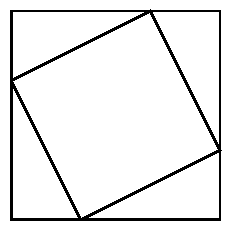
\includegraphics[height=5cm]{square-rotated}
\end{minipage}


\begin{answer}
If the larger square has side measuring $a$ units, its area is $a^2$. If the smaller square has side measuring $x$ units, its area is $x^2$. Since the side of the smaller square is the hypotenuse of the inscribed triangle, we have
\begin{align*}
x^2 = \left(\frac{a}{3}\right)^2 + \left(\frac{2a}{3}\right)^2 
    = \left(\frac{a}{3}\right)^2 (1 + 2^2) 
    = \frac{5}{9} a^2 
\end{align*}
\begin{empheq}[box={\mathbox[colback=white]}]{equation*}
    \frac{\text{outer square}}{\text{inscribed square}} = \frac{5}{9}
\end{empheq}
\end{answer}
%%%%%%%%%%%%%%%%%%%%%%%%%%%%%%%%%%%%%%%%%%%%%%%%%%%%%%%%%%%%%%%%%%%%%%%%

\iftoggle{showAnswers}{\newpage}

%%%%%%%%%%%%%%%%%%%%%%%%%%%%%%%%%%%%%%%%%%%%%%%%%%%%%%%%%%%%%%%%%%%%%%%%
\subsection*{Area of a Quadrilateral}
Quadrilateral $PSTU$ is inscribed in semicircle $O$, as shown, with $PQ=3$ units, $QR=5$ units and $RS=4$ units. What is the area of quadrilateral $PSTU$? Express your answer as a decimal to the nearest tenth. 

\begin{minipage}[b]{\linewidth}
\centering
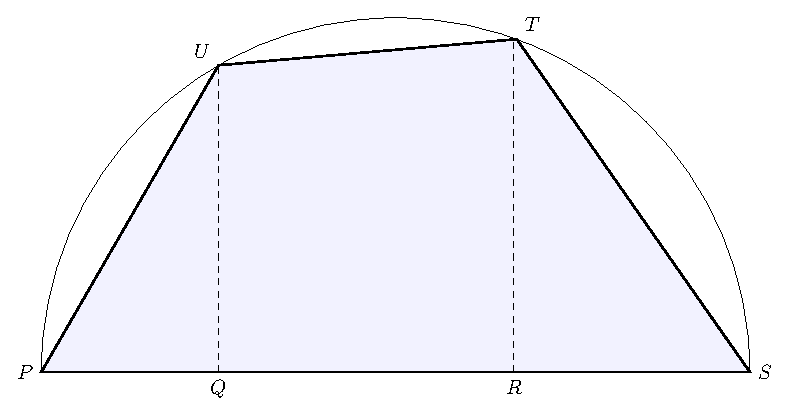
\includegraphics[height=4cm]{quadrilateral-inscribed}
\end{minipage}
\begin{answer}
One approach to calculating the area of quadrilateral $PUTS$ is to divide it into triangle $PQU$, triangle $SRT$, and trapezoid $QUTR$. A trapezoid is a quadrilateral with only one pair of parallel sides. To compute these areas, we need the heights $h_1$ and $h_2$. To calculate $h_1$, apply the Pythagoras theorem to triangle $OQU$. And likewise $h_2$ with triangle $ORT$. 
\begin{minipage}[b]{\linewidth}
\centering
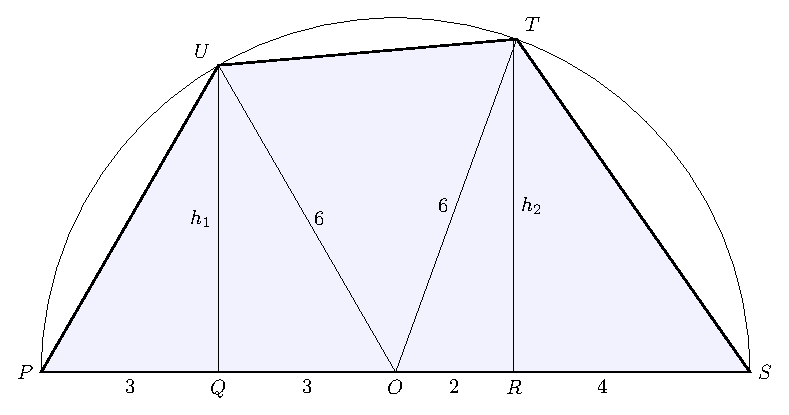
\includegraphics[height=5cm]{quadrilateral-inscribed-labeled}
\end{minipage}
\begin{align*}
h_1 & = \sqrt{6^2 -3^2} = \sqrt{27} = 3\sqrt{3} \approx 5.196 \\
h_2 & = \sqrt{6^2 -2^2} =\sqrt{32} = 4\sqrt{2} \approx 5.657
\end{align*}
The area of triangle $PQU$ and $SRT$ are:
\begin{align*}
\frac{1}{2} \times 3 \times h_1 & = 4.5\sqrt{3} \approx 7.794 \\
\frac{1}{2} \times 4 \times h_2 & = 8\sqrt{2} \approx 11.314 
\end{align*}
The area of trapezoid $QUTR$ equals the area of a parallelogram with equal base and height equal to the average height. 
\begin{align*}
QR \times \frac{h_1+h_2}{2} 
  = 5 \times \frac{3\sqrt{3}+4\sqrt{2}}{2}
  = 10\sqrt{2} + 7.5\sqrt{3}
  \approx 27.133 
\end{align*}
Adding up the areas of the triangles and trapezoid yields:
\begin{align*}
4.5\sqrt{3} + 8\sqrt{2} + 7.5\sqrt{3} + 10\sqrt{2}
  = 18\sqrt{2} + 12\sqrt{3}
  \approx 46.240
\end{align*}
\begin{empheq}[box={\mathbox[colback=white]}]{equation*}
    46.2~\text{units}^2
\end{empheq}
\end{answer}
%%%%%%%%%%%%%%%%%%%%%%%%%%%%%%%%%%%%%%%%%%%%%%%%%%%%%%%%%%%%%%%%%%%%%%%%

\iftoggle{showAnswers}{\newpage}

%%%%%%%%%%%%%%%%%%%%%%%%%%%%%%%%%%%%%%%%%%%%%%%%%%%%%%%%%%%%%%%%%%%%%%%%
\subsection*{Median in a Range}
What is the median of the integers between $1$ and $1000$ that are divisible by $28$?

\begin{answer}
There are $35$ integers divisible by $28$ in the range $[1,1000]$, since
\begin{align*}
\frac{1000}{28} \approx 35.7
\end{align*}
Since the number of integers divisible by $28$ is odd, their median is equal to the $18$th element, which is $504$, since
\begin{align*}
18 \times 28 = 504
\end{align*}
\begin{empheq}[box={\mathbox[colback=white]}]{equation*}
    504
\end{empheq}
\end{answer}
%%%%%%%%%%%%%%%%%%%%%%%%%%%%%%%%%%%%%%%%%%%%%%%%%%%%%%%%%%%%%%%%%%%%%%%%

\iftoggle{showAnswers}{\newpage}

%%%%%%%%%%%%%%%%%%%%%%%%%%%%%%%%%%%%%%%%%%%%%%%%%%%%%%%%%%%%%%%%%%%%%%%%
\subsection*{Median in a Range}
What is the median of the integers between $1$ and $1000$ that are \textit{not} divisible by $28$?

\begin{answer}
Take the range $[1,1000]$ as a starting point and consider the effect of removing the multiples of $28$. The median of the integers in the range $[1,1000]$, including the multiples of $28$, is
\begin{align*}
\frac{1000+1}{2} = 500.5
\end{align*}
There are $35$ integers divisible by $28$ in the range $[1,1000]$, of which $17$ are below the median and $18$ are above, since
\begin{align*}
\frac{1000}{28} \approx 35.7, ~~
\frac{500}{28} \approx 17.9
\end{align*}
A single deletion below the median shifts the median upwards by half a unit, while a single deletion above the median shifts it downwards by half a unit.  Removing the multiples of $28$ results in $17$ deletions below and $18$ deletions above, for an overall shift downwards of half a unit. The new median is therefore
\begin{align*}
500.5 - 0.5 = 500
\end{align*}        
\begin{empheq}[box={\mathbox[colback=white]}]{equation*}
    500
\end{empheq}
\end{answer}
%%%%%%%%%%%%%%%%%%%%%%%%%%%%%%%%%%%%%%%%%%%%%%%%%%%%%%%%%%%%%%%%%%%%%%%%

\iftoggle{showAnswers}{\newpage}

%%%%%%%%%%%%%%%%%%%%%%%%%%%%%%%%%%%%%%%%%%%%%%%%%%%%%%%%%%%%%%%%%%%%%%%%
\subsection*{Mystery Sum}
If $2015=101a+19b$, for positive integers $a$ and $b$, what is the value of $a+b$?

\begin{answer}
In complete desperation, we tried different values of $a$ until we got a hit, but there has to be a trick. To be continued...
\begin{align*}
2015 = 101 \times 16 + 19 \times 21 \\
\Rightarrow 
a = 16, b = 21
\Rightarrow 
a + b = 16 + 21 = 37
\end{align*}        
\begin{empheq}[box={\mathbox[colback=white]}]{equation*}
    a+b=37
\end{empheq}
\end{answer}
%%%%%%%%%%%%%%%%%%%%%%%%%%%%%%%%%%%%%%%%%%%%%%%%%%%%%%%%%%%%%%%%%%%%%%%%

\iftoggle{showAnswers}{\newpage}

%%%%%%%%%%%%%%%%%%%%%%%%%%%%%%%%%%%%%%%%%%%%%%%%%%%%%%%%%%%%%%%%%%%%%%%%
\subsection*{Mystery Integer}
What positive four-digit integer has its thousands and hundreds digits add up to the tens digit, its hundreds and tens digits add up to its ones digit and its tens and ones digits add up to the two-digit number formed by the thousands and hundreds digits?

\begin{answer}
Let $a$, $b$, $c$, $d$ denote the digits of the integers $abcd$, where
\begin{align*}
1 \leq a \leq 9, ~ 0 \leq b \leq 9, ~ 0 \leq c \leq 9, ~0 \leq d \leq 9
\end{align*} 
The text translates to the following set of three equations.
\begin{align*}
a + b & = c \\
b + c & = d \\
c + d & = 10a + b
\end{align*}
While these equations are linear, there are only $3$ equations for $4$ unknowns, so some clever guessing must be brought to bear on the problem. Since $a>0$ (otherwise it would not be a $4$-digit integer), the third equation implies
\begin{align*}
c + d & \geq 10
\end{align*}
In some sense, the sum $c+d$ is `large'. Meanwhile the second equation suggests that $d$ is likely to be greater than $c$ (only if $b=0$ that would not be true). So we will start to guess from $d=9$ and move down to $d=8$, $d=7$, and so on, until we hit on a solution. Thus, if $d=9$, we have:
\begin{align*}
a + b & = c \\
b + c & = 9 \\
c + 9 & = 10a + b \\
\Rightarrow a = 1, b = 4, c = 5, d = 9
\end{align*}
We hit a solution on our first attempt!
\begin{empheq}[box={\mathbox[colback=white]}]{equation*}
    1459
\end{empheq}
\end{answer}
%%%%%%%%%%%%%%%%%%%%%%%%%%%%%%%%%%%%%%%%%%%%%%%%%%%%%%%%%%%%%%%%%%%%%%%%

\iftoggle{showAnswers}{\newpage}

%%%%%%%%%%%%%%%%%%%%%%%%%%%%%%%%%%%%%%%%%%%%%%%%%%%%%%%%%%%%%%%%%%%%%%%%
\subsection*{Based On 2021 Chapter Invitational Sprint Q29.}
Square ABCD, shown here, has side length $a$ units. Points P and Q are located on sides AD and BC, respectively, with $\text{AP}=\text{BQ}=b$ units. Triangles ACP and BDQ overlap in the square to form the shaded quadrilateral. What is the area of the shaded quadrilateral? Express your answer as a common fraction. 

\begin{center}
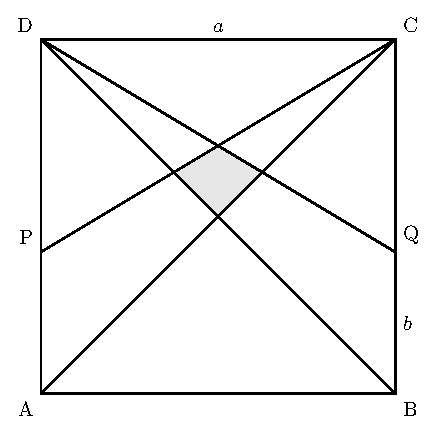
\includegraphics[height=10cm,page=1]{quadrilateral-area-shaded}
\end{center}

\begin{answer}
For clarity, add labels to the shaded quadrilateral: 
\begin{center}
\includegraphics[height=5cm,page=2]{quadrilateral-area-shaded}
\end{center}
The area of the quadrilateral NESW is equal to half the product of its diagonals, NS and ES. If we denote by $h$ the vertical diagonal NS, or `height', and by $w$ the horizontal diagonal EW, or `width', the area is given by:
\begin{align*}
\frac{wh}{2}
 = 
\frac{\text{EW} \times \text{NS}}{2}
\end{align*}
where S is the intersection of the diagonals of the square ABCD (the center of the square), and N is the intersection of the diagonals of the rectangle CDPQ.

The height of the quadrilateral follows immediately from the ``Intercept Theorem''. The Intercept theorem states that Given two parallel lines AC and BD and some point S, the following ratios hold:
\begin{align*}
\frac{\text{SA}}{\text{SB}} 
  = \frac{\text{SC}}{\text{SD}} 
  = \frac{\text{AC}}{\text{BD}} 
\end{align*} 
\begin{center}
\includegraphics[height=6cm,page=6]{quadrilateral-area-shaded}
\end{center}

Applying the Intercept Theorem to point D and the parallel lines NS and QB gives:
\begin{align*}
\frac{\text{DQ}}{\text{DN}} 
  = \frac{\text{DB}}{\text{DS}} 
  = \frac{\text{QB}}{\text{NS}} 
\end{align*}
and since $\text{DB}=2\text{DS}$ (the center of the square S cuts the diagonal DB in half) and $\text{QB}=b$ (as stated in the question), it follows that the height of the quadrilateral is
\begin{align*}
h = \text{NS} = \frac{b}{2}
\end{align*}
\begin{center}
\includegraphics[height=10cm,page=3]{quadrilateral-area-shaded}
\end{center}
Next, we calculate the width of the quadrilateral. Let $w$ denote the length of EW and let $x$ denote the length of $\text{E}\text{E}^{\prime}$. Since the square has side length $a$, we have $x+w+x=a$ (see the figure), or $w=a-2x$. Thus, $w$ follows from $x$: it is easier to calculate $x$. 
\begin{center}
\includegraphics[height=10cm,page=4]{quadrilateral-area-shaded}
\end{center} 

It is easier to calculate $x$ than $w$, because the existence of a square of side length $x$ allows us to change perspective. Earlier we found it quite straightforward to calculate the vertical distance $h$ by applying the Intercept theorem, because of the existence of two parallel lines intersecting an angle at known distances. Applying similar reasoning to $w$ leads us to consider triangle CSD and the parallel lines EW and DC (see figure below). Unfortunately, the distances needed to apply the Intercept theorem are not immediately known. By contrast, applying similar reasoning to $x$ gives several ways to apply the Intercept theorem. We could consider triangle DQC and the parallel lines $\text{E}\text{E}^{\prime}$ and DC. Or we could consider triangle CDQ and the parallel lines $\text{E}^{\prime\prime}\text{E}$ and CQ. 

\begin{center}
\includegraphics[height=10cm,page=8]{quadrilateral-area-shaded}
\end{center} 


Consider triangle CDQ. Because CE is on the diagonal of square ABCD, it is a bisector of DCQ, and therefore it is the diagonal of square $\text{C}\text{E}^{\prime}\text{E}\text{E}^{\prime\prime}$. Thus, the lengths of $\text{C}\text{E}^{\prime\prime}$ and $\text{E}\text{E}^{\prime}$ are equal, implying that triangles CDQ and  $\text{E}^{\prime\prime}\text{D}\text{E}$ are similar. For two similar triangles, the ratio of their legs are equal, for instance:
\begin{align*}
\frac{\text{C}\text{D}}{\text{C}\text{Q}} 
= \frac{\text{E}^{\prime\prime}\text{D}}{\text{E}^{\prime\prime}\text{E}}  
\end{align*}
Focusing on triangle CDQ makes this clearer:
\begin{center}
\includegraphics[height=8cm,page=5]{quadrilateral-area-shaded}
\end{center}
From $\text{CD}=a$, $\text{CQ}=a-b$ and   $\text{C}\text{E}^{\prime\prime}=\text{E}^{\prime\prime}\text{E}=\text{E}\text{E}^{\prime}=x$, we get $\text{E}^{\prime\prime}\text{D}=CD-\text{C}\text{E}^{\prime\prime}=a-x$. Substituting known lengths into the above relation yields an equation in $x$:
\begin{align*}
\frac{a}{a-b} = \frac{a-x}{x} 
\end{align*}
which may be solved for $x$ in terms of $a,b$, from which $w$ follows: 
\begin{align*}
x & = \frac{a(a-b)}{2a-b} \\
w & = a - 2x 
    = a - 2 \times \frac{a(a-b)}{2a-b} 
    = \frac{a(2a-b)-2a(a-b)}{2a-b}
    = \frac{ab}{2a-b}
\end{align*}
The area of the quadrilateral is then:
\begin{align*}
\frac{b}{2} \times \frac{ab}{2(2a-b)}
  = \frac{ab^2}{4(2a-b)}
\end{align*}
In the special case $a=6$ and $b=1$ (the values in the Chapter Invitational), the area is
\begin{align*}
\frac{ab^2}{4(2a-b)}
 = \dfrac{3}{22}~\text{units}^{2}
\end{align*}

\newpage 
In a solution provided in association with MathCounts, Prof. Po Shen Loh showed a different approach to calculate $w$, somewhat easier and faster. Consider the system of Cartesian coordinates centered at point A, with $x$-axis along AB and $y$-axis along AD. In this system, diagonal AC has equation $y=x$ (the $45^{\circ}$ line), while line DQ has equation
\begin{align*}
y = a - \frac{a-b}{a} x
\end{align*}
The intercept is obviously $a$ (the side length AD), while the slope is the vertical displacement, $-(a-b)$ (length of segment CQ, with a negative sign to mark the descent), divided by the horizontal displacement, $a$ (length of segment DC).
\begin{center}
\includegraphics[height=12cm,page=7]{quadrilateral-area-shaded}
\end{center}
Half the width of the quadrilateral is then the $x$-coordinate of point E minus the $x$-coordinate of the center of the square. Thus,
\begin{align*}
w = 2\left(x_{\text{E}} - \frac{a}{2}\right)
\end{align*}

The value of $x_{\text{E}}$ is found by solving the system:
\begin{align*}
\begin{cases}
y ~= & x \\
y ~= & a - \dfrac{a-b}{a} x
\end{cases}
\end{align*}
which yields $w$ once again:
\begin{align*}
x_{\text{E}} = \frac{a^2}{2a-b}, 
  \quad
w = 2\left(x_{\text{E}} - \frac{a}{2}\right)
  = 2 \left(\frac{a^2}{2a-b}-\frac{a}{2}\right)
  = \frac{2a^2-a(2a-b)}{2a-b}
  = \frac{ab}{2a-b}
\end{align*}
\end{answer}
%%%%%%%%%%%%%%%%%%%%%%%%%%%%%%%%%%%%%%%%%%%%%%%%%%%%%%%%%%%%%%%%%%%%%%%%

\iftoggle{showAnswers}{\newpage}

%%%%%%%%%%%%%%%%%%%%%%%%%%%%%%%%%%%%%%%%%%%%%%%%%%%%%%%%%%%%%%%%%%%%%%%%
\subsection*{Four Equilateral Triangles}
If $a$ is the side length of one of the four equilateral triangles, calculate the shaded area. 

\begin{center}
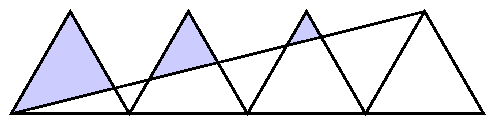
\includegraphics[height=4cm,page=1]{four-triangles-areas}
\end{center}

\begin{answer}
First, consider the red triangle below. 
\begin{center}
\includegraphics[height=4cm,page=2]{four-triangles-areas}
\end{center}

Next, consider a second triangle below. The legs divide the $\delta$ line into four segments of equal length. By the intercept theorem, the parallel line in the middle has length $\frac{a}{2}$. By the same reasoning, the shorter line has length half of that, or $\frac{a}{4}$. And likewise, the longer line has length three times that, or $\frac{3a}{4}$.
\begin{center}
\includegraphics[height=4cm,page=3]{four-triangles-areas}
\end{center}

To sum up, we have the following:
\begin{center}
\includegraphics[height=4cm,page=4]{four-triangles-areas}
\end{center}

Still with the same triangle, similar considerations yield lengths for the opposite legs:
\begin{center}
\includegraphics[height=4cm,page=5]{four-triangles-areas}
\end{center}

Since the three shaded triangles are similar, the relative leg lengths can be used to calculate the relative areas. That is, if $A$ denotes the area of the larger triangle, then the middle triangle has area $(2/3)^2A$ and the small triangle area $(1/3)^2A$.
\begin{center}
\includegraphics[height=4cm,page=6]{four-triangles-areas}
\end{center}
The sum of the three areas in terms of $A$ is therefore:
\begin{align*}
A + \frac{4A}{9} + \frac{A}{9}
 = \frac{9+4+1}{9} A
 = \frac{14}{9} A
\end{align*}
Up to this point, the reasoning and calculations were fairly straightforward.

Knowing the side lengths $a$, $b=3a/4$, and $c=\delta/4$, we could calculate area $A$ by applying Heron's formula. First, calculate $\delta$  by applying Pythagoras:
\begin{align*}
\delta 
  & = \sqrt{%
    \left(3a + \frac{a}{2}\right)^2 
  + \left(\frac{\sqrt{3}}{2}\right)^2 
  } 
  = \frac{\sqrt{7^2+3}}{2} a
  = \sqrt{13} a
\end{align*}

This gives $c=\delta/4=\sqrt{13}a/4$. Unfortunately, applying Heron's formula is tedious and prone to errors: 
\begin{align*}
s & = \frac{a+b+c}{2}
    = \frac{a + \frac{3a}{4} + \frac{\sqrt{13}a}{4}}{2} \\
A & = \sqrt{s(s-a)(s-b)(s-c)}
    = \sqrt{s\left(s-a\right)\left(s-\frac{3a}{4}\right)\left(s-\frac{\sqrt{13}a}{4}\right)}
\end{align*}
An easier way to calculate $A$ follows from two considerations. First, the area of an equilateral triangle of side length $a$ is 
\begin{align*}
\frac{\sqrt{3}}{4} a^2
\end{align*}
This is a well-known result that follows from an application of the Pythagorean theorem. Secondly, the area of the shaded portion $A$ is simply three-quarters of the whole. This follows from the side length being $(3/4)a$: 
\begin{center}
\includegraphics[height=4cm,page=7]{four-triangles-areas}
\end{center}
Putting it together:
\begin{align*}
A = \frac{3}{4} \times \sqrt{3}\left(\frac{a}{2}\right)^2
  = \frac{3\sqrt{3}}{16} a^2
\end{align*}

The total area is therefore:
\begin{align*}
\frac{14}{9}  A 
  = \frac{14}{9} \times \frac{3}{4} \times \frac{\sqrt{3}}{4} a^2
  = \frac{7\sqrt{3}}{24} a^2
\end{align*}

In one variant of the problem we are given that the area of the equilateral triangle is $6$ units:
\begin{align*}
\frac{\sqrt{3}}{4} a^2 = 6
\end{align*} 
and so in this special case the total area is $7$ units$^2$: 
\begin{align*}
\frac{14}{9} \times \frac{3}{4} \times 6
  = 7
\end{align*}

\end{answer}


\iftoggle{showAnswers}{\newpage}

%%%%%%%%%%%%%%%%%%%%%%%%%%%%%%%%%%%%%%%%%%%%%%%%%%%%%%%%%%%%%%%%%%%%%%%%
\subsection*{A Circle Packing Problem}
The problem presented here was originally proposed by Batsui Mitsunao, a fifteen-year-old boy, and written on a tablet hung in 1812 at the Nishihirokami Hachiman shrine in Izumi city, Toyama prefecture, Japan (Fukagawa Hidetoshi and Tony Rothman, \textit{Sacred Mathematics: Japanese Temple Geometry}, Princeton University Press, 2008). 

Several circles of radius $r$ are packed to form a pyramid, using $n$ circles along each side, as shown in the figure below in the special case $n=4$. A larger circle circumscribes the pyramid. Express the radius of the larger circle in terms of $r$ and $n$. Express the ratio of the areas of the $n$ smaller circles to the area of the larger circle in terms of $n$. Calculate the limit of the ratio as $n\rightarrow\infty$. 


\begin{center}
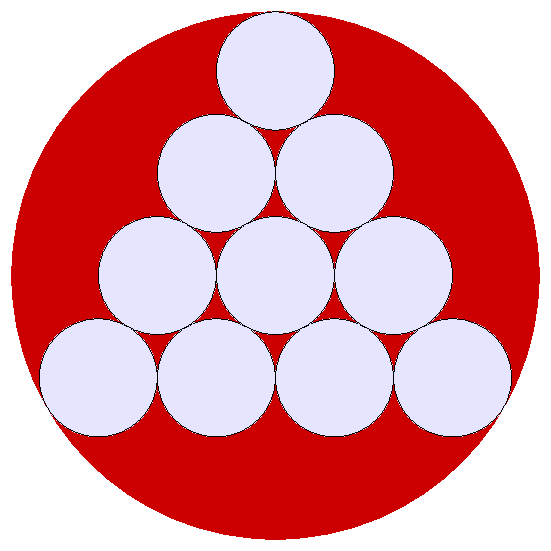
\includegraphics[height=6cm,page=1]{circles-in-pyramid}
\end{center}

\begin{answer}
Consider the equilateral triangle formed by connecting the centers of the three circles positions at the far east/west/north positions. The center of the triangle --- the point where the three bisectors intersect --- is also the center of the large circle. Let $a$ denote the side length of the triangle. Let $x$ denote the distance from one vertex to the center of the triangle. The height of the triangle is $x+y$. See the figure below. 
\begin{center}
\includegraphics[width=0.45\linewidth,page=2]{circles-in-pyramid}%
\includegraphics[width=0.45\linewidth,page=3]{circles-in-pyramid}
\end{center}
Let $R$ denote the radius of the larger circle. Then $R=x+r$. We want to express $x$ in terms of $r$ and $n$. To do this, we first express $x$ in terms of $a$ and then express $a$ in terms of $r$ and $n$. The relation between $x$ and $a$ for an equilateral triangle is well known; it is not difficult to calculate it by applying the Pythagorean theorem (see below). We state it here: 
\begin{align*}
x = \frac{\sqrt{3}a}{3}
\end{align*}
We can express $a$ in terms of $r$ and $n$ as follows. The circle's centers are a distance $r$ from the circle. The distance between two centers is equal to the diameter multiplied by the number of circles, or $n-2$. This gives a side length of $r + 2r(n-2) + r$ (adding lengths from one end to the other) and thus
\begin{align*}
a =  2r(n-1)
\end{align*}
Substituting back into $x$ gives
\begin{align*}
x = \frac{2\sqrt{3}(n-1)r}{3}
\end{align*}
The radius of the larger circle $R=r+x$ is therefore 
\begin{align*}
R = \frac{\left(3+2\sqrt{3}(n-1)\right)r}{3}
\end{align*}

The pyramid's base has $n$ circles, the next row above $n-1$, the one above $n-2$, and so on until the top row with $1$ circle. The total number of circles is therefore:
\begin{align*}
n + (n-1) + (n-2) + \ldots + 1
  = \frac{n(n+1)}{2}
\end{align*}

The area of one small circle is $\pi r^2$. The ratio of the areas occupied by the small circles to the area of the larger circle is:
\begin{align*}
\frac{\dfrac{n(n+1)}{2} \pi r^2}{\pi R^2}
 & = 
\frac{\dfrac{n(n+1)}{2}}{\dfrac{\left(3+2\sqrt{3}(n-1)\right)^2}{3^2}}\\[1em]
 & = 
\dfrac{9n(n+1)}{2\left(3+2\sqrt{3}(n-1)\right)^2}\\[1em]
 & = 
\dfrac{3n(n+1)}{2\left(3+4\sqrt{3}(n-1)+4(n-1)^2\right)}
\end{align*}

How does this ratio depend on $n$? The figure below shows the percentage of the larger circle's area filled by the small circles for several values of $n$. 
\begin{center}
\includegraphics[width=\linewidth,page=6]{circles-in-pyramid}
\end{center}
As $n$ gets larger, the ratio tends to:
\begin{align*}
\frac{3n(n+1)}{8(n-1)^2} \rightarrow \frac{3}{8}
~\text{as}~n\rightarrow\infty
\end{align*}
How does this compare to the ratio of the area of the triangle to the area of the larger circle? The area of the triangle is:
\begin{align*}
%\frac{a(x+y)}{2} = 
\frac{\sqrt{3}a^2}{4}
  = \sqrt{3}(n-1)^2r^2
\end{align*}
And therefore the ratio of areas:
\begin{align*}
\frac{\sqrt{3}(n-1)^2r^2}{\dfrac{\pi\left(3+2\sqrt{3}(n-1)\right)^2r^2}{3^2}}
= \frac{3\sqrt{3}(n-1)^2}{\pi\left(3+4\sqrt{3}(n-1)+4(n-1)^2\right)}
\rightarrow \frac{3\sqrt{3}}{4\pi}~\text{as}~n\rightarrow\infty
\end{align*}

In the limit, as the number of smaller circles becomes arbitrarily large, $n\rightarrow\infty$, the area covered by the circles tends to $0.375$, while the area of the triangle is approximately $0.413$, about $10$ percent larger. 

We now show how to calculate $x$ in an equilateral triangle of side length $a$. We first calculate the height of the triangle. Let $h$ denote the height:
\begin{center}
\includegraphics[height=5cm,page=7]{circles-in-pyramid}
\end{center}

Apply the Pythagorean theorem to find the height $h$:
\begin{align*}
& \left(\frac{a}{2}\right)^2 + h^2 = a^2 \\
\Rightarrow 
& h = \frac{\sqrt{3}a}{2}
\end{align*}

Split the height into two parts, $h=x+y$:
\begin{center}
\includegraphics[height=5cm,page=3]{circles-in-pyramid}
\end{center}
Apply the Pythagorean theorem and eliminate $y$ by substituting $y=h-x$:
\begin{align*}
& \left(\frac{a}{2}\right)^2 + y^2 = x^2 \\
\Rightarrow \quad
& \left(\frac{a}{2}\right)^2 + \left(\frac{\sqrt{3}a}{2}-x\right)^2 = x^2 \\
\Rightarrow \quad
& \left(\frac{a}{2}\right)^2 + 3 \left(\frac{a}{2}\right)^2 - \sqrt{3}ax + x^2 = x^2 \\[1em]
\Rightarrow \quad
& x = \dfrac{4\left(\dfrac{a}{2}\right)^2}{\sqrt{3}a} \\[1em]
\Rightarrow \quad
& x = \frac{\sqrt{3}a}{3}
\end{align*}
With $h$ and $x$, we can also calculate $y = \dfrac{\sqrt{3}a}{6}$.

\end{answer}


\end{document}




%%%%%%%%%%%%%%%%%%%%%%%%%%%%%%%%%%%%%%%%%%%%%%%%%%%%%%%%%%%%%%%%%%%%%%%%
\subsection*{Mystery Pattern}
Can you find the pattern?
\begin{minipage}[b]{\linewidth}
\centering
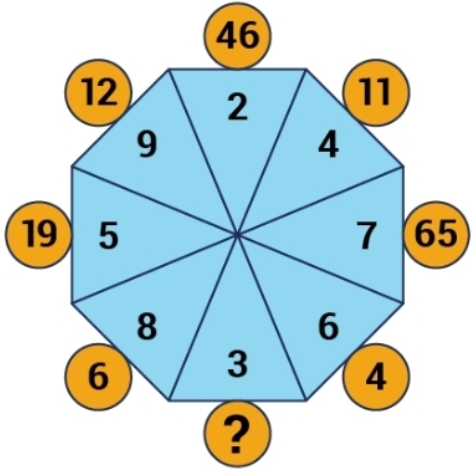
\includegraphics[height=6cm]{pattern-guess}
\end{minipage}
%%%%%%%%%%%%%%%%%%%%%%%%%%%%%%%%%%%%%%%%%%%%%%%%%%%%%%%%%%%%%%%%%%%%%%%%
